\subsection{扩张}

定义 5. 设 \(\mathfrak{a}\) 和 \(\mathfrak{b}\) 是 \(\mathbf{K}\) 上的两个李代数。\(\mathfrak{b}\) 的 \(\mathfrak{a}\)-扩张是一个序列：

\[
a \xrightarrow {\lambda} g \xrightarrow {\mu} b
\]

其中 g 是 K 上的李代数，μ 是从 g 到 b 的满同态，λ 是将 a 同构到 μ 的核上的单同态。

扩张的核称为 \(\mathfrak{n}\)，即 \(\mu\) 的核。取商后，同态 \(\lambda\) 将 \(\mathfrak{a}\) 同构到 \(\mathfrak{n}\) 上，而同态 \(\mu\) 定义了从 \(\mathfrak{g} / \mathfrak{n}\) 到 \(\mathfrak{b}\) 的同构。

滥用术语，也称 g 为由 a 扩张 b。

两个扩张：

\[
a \xrightarrow {\lambda} g \xrightarrow {\mu} b, \quad a \xrightarrow {\lambda^ {\prime}} g ^ {\prime} \xrightarrow {\mu^ {\prime}} b
\]

若存在一个同态 \(f\)，它从 \(\mathfrak{g}\) 到 \(\mathfrak{g}'\)，使下图：

\pandocbounded{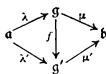
\includegraphics[keepaspectratio]{images/part001_2862d8fe.jpg}}

是交换的（即满足 \(f \circ \lambda = \lambda', \mu' \circ f = \mu\)），则称这两个扩张等价。我们说明这样的同态必为双射。首先 \(f\) 是单射。若 \(x \in \mathfrak{g}\) 满足 \(f(x) = 0\)，则 \(\mu(x) = \mu'(f(x)) = 0\)，从而 \(x = \lambda(y)\)，其中某个 \(y \in \mathfrak{a}\)；于是 \(\lambda'(y) = f(\lambda(y)) = f(x) = 0\)，故 \(y = 0\)，进而 \(x = 0\)。另一方面，\(f\) 是满射。因为 \(\mu' \circ f = \mu\) 是满射，所以 \(f(\mathfrak{g}) + \lambda'(\mathfrak{a}) = \mathfrak{g}'\)；另一方面 \(f(\mathfrak{g}) \supset f(\lambda(\mathfrak{a})) = \lambda'( \mathfrak{a})\)。

由此可知，刚才定义的两个由 a 扩张 b 之间的关系是等价关系。

命题 6. 设

\[
a \xrightarrow {\lambda} g \xrightarrow {\mu} b
\]

是由 a 扩张 b 的扩张，n 是其核。

\begin{enumerate}
\def\labelenumi{(\alph{enumi})}
\item
  若 g 有一个在 g 中补 n 的子代数 m，则 μ 在 m 上的限制是从 m 到 b 的同构。若 v 表示此限制的逆同构，则 v 是从 b 到 g 的同态，且 μ ∘ v 是 b 的恒等自同构。
\item
  反之，若存在一个同态 \(v\)，它从 \(\mathfrak{b}\) 到 \(\mathfrak{g}\)，使 \(\mu \circ v\) 是 \(\mathfrak{b}\) 的恒等自同构，则 \(v(\mathfrak{b})\) 是 \(\mathfrak{n}\) 在 \(\mathfrak{g}\) 中的补子代数。
\end{enumerate}

（a）的断言是直接的。另一方面，设 v 是从 b 到 g 的同态，且 \(\mu \circ v\) 是 b 的恒等自同构。则 \(v(b)\) 是 g 的子代数，并且 g 是 \(v(b)\) 与 \(\mu^{-1}(0) = n\) 的直和（Algebra, Chapter VIII, §1, no. 1）。

定义 6. 设

\[
a \xrightarrow {\lambda} g \xrightarrow {\mu} b
\]

是一个 \(\mathfrak{b}\) 的 \(\mathfrak{a}\)-扩张，\(\mathfrak{n}\) 是其核。如果 \(\mathfrak{g}\) 中存在一个子代数（分别为理想）补 \(\mathfrak{n}\) 于 \(\mathfrak{g}\)，则称此扩张为非本质的（分别为平凡的）。若 \(\mathfrak{n}\) 包含于 \(\mathfrak{g}\) 的中心，则称此扩张为中心扩张。

若扩张是平凡的，设 \(m\) 是 \(g\) 中补 \(n\) 于 \(g\) 的理想。则（参见第 1 号）\(g\) 自然地与李代数 \(m \times n\) 相同，因而也与李代数 \(a \times b\) 相同。反之，设 \(a\) 和 \(b\) 是两个李代数，则 \(a \times b\) 是 \(b\) 的 \(a\)-平凡扩张。

非本质的中心扩张是平凡的。事实上，设 \(\mathfrak{g}\) 是李代数，\(\mathfrak{n}\) 是包含于 \(\mathfrak{g}\) 中心的 \(\mathfrak{g}\) 的理想，\(\mathfrak{m}\) 是 \(\mathfrak{g}\) 中补 \(\mathfrak{n}\) 于 \(\mathfrak{g}\) 的子代数。则 \([\mathfrak{m},\mathfrak{g}] = [\mathfrak{m},\mathfrak{m}] + [\mathfrak{m},\mathfrak{n}] = [\mathfrak{m},\mathfrak{m}] \subset \mathfrak{m}\)，所以 \(\mathfrak{m}\) 是 \(\mathfrak{g}\) 的理想。

